\documentclass{report}

\usepackage{textcomp}
\usepackage{graphicx}
\usepackage{fancyhdr}
\usepackage{subcaption}
\usepackage{multicol}
\usepackage{outlines}
%===================================
\newcommand{\classinfo}{{\bf Legacy Inter-Vlan \\ Implementation}\\{\it CIT 167}\\{Chaz Davis}}
\newcommand{\semester}{BCTC \\ Spring 2020}
%===================================
\newcommand{\mysection}[1]{\section*{#1}}
\newcommand{\mysubsection}[2]{\textbf{\romannumeral #1) #2}}
%===================================
\setlength{\headheight}{15.2pt}
\pagestyle{fancy}
\fancyhf{}
\lhead{ \fancyplain{}{Chaz Davis} }
\rhead{ \fancyplain{}{\today} }
\cfoot{ \fancyplain{}{\thepage} }
\renewcommand{\headrulewidth}{0.5pt}
\renewcommand{\footrulewidth}{0pt}

%===================================
\title{\classinfo}
\author{\semester}
\date{\today}

%===================================

\begin{document}

\maketitle

%===================================
\mysection{\textbf{Part 1: Configuring and verifying the network}}

I setup the Configuration according to the handout. I then, configured the IP
address, default gateways, and subnet masks on each of the PCs.
I Next ran the commands on R1, and then the commands on S1. I had to go back
and run {\scriptsize{\verb$int g0/1 no shut$}\normalsize} on R1.

After that I was able to successfully ping from PC1 to PC3.


\begin{figure}[!hbt]\centering
\subfloat[Pinging from PC1 to
PC3]{\label{success14ping}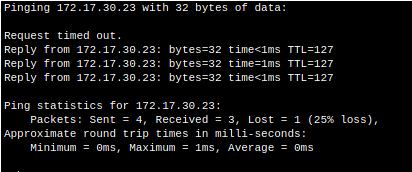
\includegraphics[width=.45\linewidth]{Figures/2020-03-08-194333_412x172_scrot.png}}\par
\subfloat[Successful network
architecture]{\label{success14arch}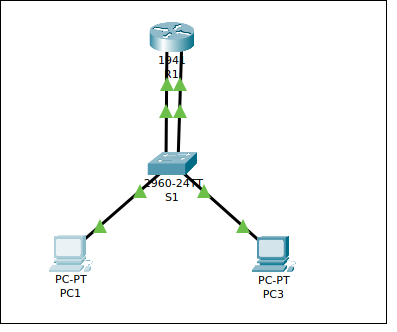
\includegraphics[width=.45\linewidth]{Figures/2020-03-08-194344_397x332_scrot.png}}\par
\caption{Successful Lab layout}
\label{success14}
\end{figure}








%===================================

\end{document}
